\subsection{実験3 ロボットマニピュレータ軌道予測問題における速度変化に対するモデル精度評価}
提案手法をロボットマニピュレータ手先軌道予測問題に適用し, 軌道速度変化に対するモデル精度評価を行う.

\subsubsection{実験環境}
実験環境は物理シミュレータであるMujoco\cite{mujoco}を用いた.
また, ロボットマニピュレータは6つの自由度を持つUR5eを用いた.
UR5eの構成図とDenavit-Hartenbergパラメータ (DHパラメータ)をそれぞれ\figref{fig:ur5e:structure}と\tabref{tab:ur5e:dh}に示す\cite{ur5e}.
UR5eの制御は目標手先位置から目標関節角度を逆運動学で求め, PD制御によって行った.
ここで, PD制御におけるPゲイン$K_p$, Dゲイン$K_d$はそれぞれ$1$, $0.1$とした.
また, 目標関節角度の計算はMujocoにおける微分運動学ライブラリであるmink\cite{mink}を用いた.
\begin{figure}[htbp]
    \centering
    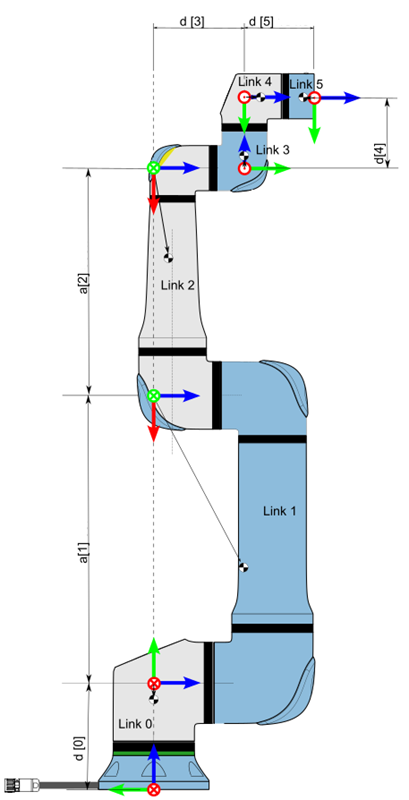
\includegraphics[width=0.5\textwidth]{Static/ur5e_structure.png}
    \caption{UR5eの構成図}
    \label{fig:ur5e:structure}
\end{figure}

\begin{table}[htbp]
    \centering
    \caption{UR5eのDHパラメータ}
    \label{tab:ur5e:dh}
    \begin{tabular}{ccccc}
        \hline
        \textbf{Joint} & $\bm{\theta}$ [rad] & $\bm{a}$ [m]& $\bm{d}$ [m]& $\bm{\theta}$ [rad]\\
        \hline
        1 & 0 & 0       & 0.1625 & $\pi/2$\\
        2 & 0 & -0.425  & 0       & 0\\
        3 & 0 & -0.3922 & 0       & 0\\
        4 & 0 & 0       & 0.1333 & $\pi/2$\\
        5 & 0 & 0       & 0.0997 & $-\pi/2$\\
        6 & 0 & 0       & 0.0996 & 0\\
        \hline
    \end{tabular}
\end{table}

